\item You are hired by a moving company to move $N$ boxes from a corner of a room to the opposite
corner of the room. The room can be roughly divided into four corners, and there is an indoor
pond in the middle of the room preventing any direct diagonal crossing. The three boxes have
different sizes and can only be stacked in such a way that larger boxes can never be placed
on top of smaller ones.\\
Please answer the following questions:
\begin{enumerate}
  \item Given $N$ boxes (stacked appropriately in corner $A$ with the smallest box on the top), formulate this problem as a search problem. Indicate the
        \begin{itemize}
          \item States (describe specifically what a state is in this problem, how you would store it in a computer using a data structure, and justify the correctness of your representation)
          \item Actions
          \item Cost of different actions
          \item Successor state for each action and give one example with all of its successor states listed
          \item The objective
        \end{itemize}
        I made some assumptions for this problem:
        \begin{itemize}
          \item I can only move one box at a time
          \item I can only remove a box from the top of a stack
          \item I can only add a box to the top of a stack
          \item I cannot sort a stack in place
          \item Each room can only contain one stack
          \item All boxes have unique sizes
          \item All stacks must be appropriately placed, smallest box at top largest at bottom
        \end{itemize}
        With the rules of the game clear, we can define the state unambiguously.\\
        Let the set of rooms be $R = \{a, b, c, d\}$, a box $B$ with size $i$ be $b_i\in B=\{b_1, b_2, \ldots ,b_n\}$, a stack $G$ in room $r$ be $g(r) \subseteq B$ and a box $b_i$ in a stack $g(r)$ be $g(r,i)\in B$, the number of boxes be $N$, and the position of the mover $M$ in the room $r$ be $M = m_r$.\\
        We can then represent the start state as with $N=3$ as
        \begin{align*}
          g(a) & = \{b_1, b_2, b_3\} \\
          g(b) & = \{\emptyset\}     \\
          g(c) & = \{\emptyset\}     \\
          g(d) & = \{\emptyset\}     \\
          M    & = m_a
        \end{align*}
        And the goal state as the state where all boxes are in $g(d)$
        \begin{align*}
          g(a) & = \{\emptyset\}     \\
          g(b) & = \{\emptyset\}     \\
          g(c) & = \{\emptyset\}     \\
          g(d) & = \{b_1, b_2, b_3\} \\
          M    & = m_d
        \end{align*}
        This represents 4 stacks $g(r)$ in each room $R = \{a, b, c, d\}$, with a set of boxes. Each stack must be ordered from smallest to largest. And $M$ represents the position of the mover.\\
        To represent the state as a data structure in Python, we can use a list containing 4 stacks. Each stack represents the stack of boxes in a room. We can assign each room to each stack respectively in increasing order. The stack is implemented as an integer list and each integer represents the size of a box. The mover can be represented as a separate integer variable containing the index of the stack he is in. Here is a diagram to illustrate this model.
        \begin{center}
          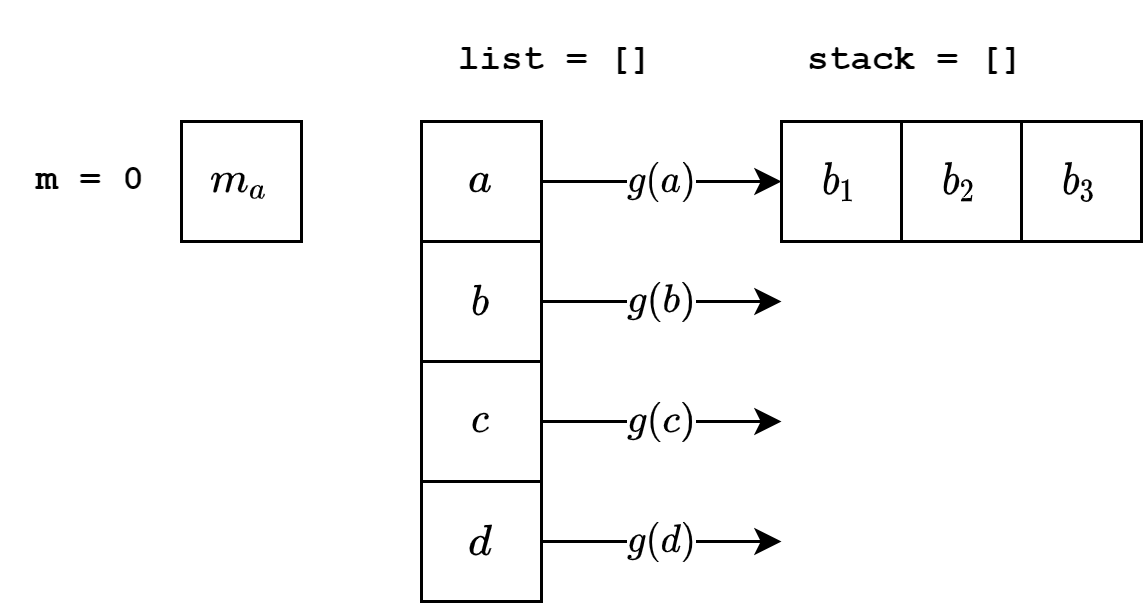
\includegraphics[scale=0.3]{"./Diagrams/Q2_DataStructure.png"}
        \end{center}
        This data structure is correct because it contains all possible positions of the boxes in every room. It also contains all possible rooms the mover can be in. It does not enforce the constraints such as the ordering or the diagonal constraint. These will be enforced by the methods we are allowed to perform on the data structure.\\
        The base action in our system is to move a box from one room to an adjacent room, subject to the system rules. This action has a cost 1. We further simplify the actions by assuming that:
        \begin{itemize}
          \item The size of the box doesn't affect the cost
          \item Moving without a box has 0 cost
          \item Appending and popping from a stack (picking up and putting down a box) costs 0
          \item Mover must be in the same room as a box to pick up or put down a box
        \end{itemize}
        For example, for an action $C(a, b), C(b, d)$ represents popping a box from the top of the stack $g(a)$ and carrying it to room $b$, then carrying it to room $d$ and appending it to the top of the stack $g(d)$. The popping and appending costs 0. The moving has a cost of $1+1=2$ as we travelled from $a\rightarrow b$ and from $b\rightarrow d$. In the implementation, there must be checks to ensure that the ordering rule is respected when appending to a stack.\\
        Here is an example of a state with $N=1$ and all successor states.
        \begin{center}
          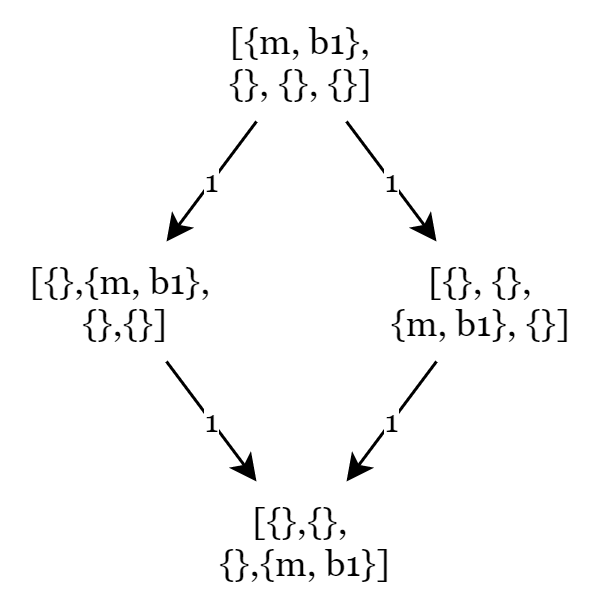
\includegraphics[scale=0.4]{"./Diagrams/Q2_StartStateWithAllSuccessorStates.png"}
        \end{center}
        This represents a start state where one box $b_1$ is in room $a$ and the mover is also in room $a$. The possible actions from the start state are to move the box to rooms $b$ or $c$, then to $d$.\\
        We can see that we have reached the goal state by completing action in two steps as all the boxes are in the room $d$.
  \item For using heuristic search methods such as A*, provide an admissible heuristic and justify why it is admissible.\\[10pt]
        An admissible heuristic for some state $n$ would be the number of boxes not in room $d$.
        $$
          h(n) = N - \lvert g(d)\rvert
        $$
        Given a base case where we have a single box in room $b$, the least cost path is 1, which is to take the box directly to $C(b,d)$. But for any other case where we have more than 1 box or if our box is located diagonally from the $d$, the cost would be greater as we cannot directly append the boxes to stack $g(d)$ as it will violate the ordering rule. We might also have to travel more than one room to reach $d$.\\
        This will always result in a cost greater than the heuristic.Thus the heuristic admissible.
  \item For the case where $N = 3$, compute the first three steps of DFS search. You can use the table structure as in question 1c to show different steps.
        \begin{center}
          \bgroup
          \def\arraystretch{1.5}%
          \begin{tabular}{|c|c|}
            \hline
            Step \# & Stacks                                    \\
            \hline
            $1$     & $[\{m,b_1, b_2, b_3\}, \{\}, \{\}, \{\}]$ \\
            $2$     & $[\{b_2, b_3\}, \{m,b_1\}, \{\}, \{\}]$   \\
            $3$     & $[\{m,b_2, b_3\}, \{b_1\}, \{\}, \{\}]$   \\
            \hline
          \end{tabular}
          \egroup
        \end{center}
  \item Give a solution to the problem for $N = 3$. You can achieve it either using some methods from the class or through guessing.
        I am ignoring the position of the mover $m$ in the state here as his movement without a box costs 0. To transition from a state $[\{b_2, b_3\}, \{m,b_1\}, \{\}, \{\}]$ to $[\{m,b_2, b_3\}, \{b_1\}, \{\}, \{\}]$ costs 0, so I will omit it for brevity's sake.
        \begin{center}
          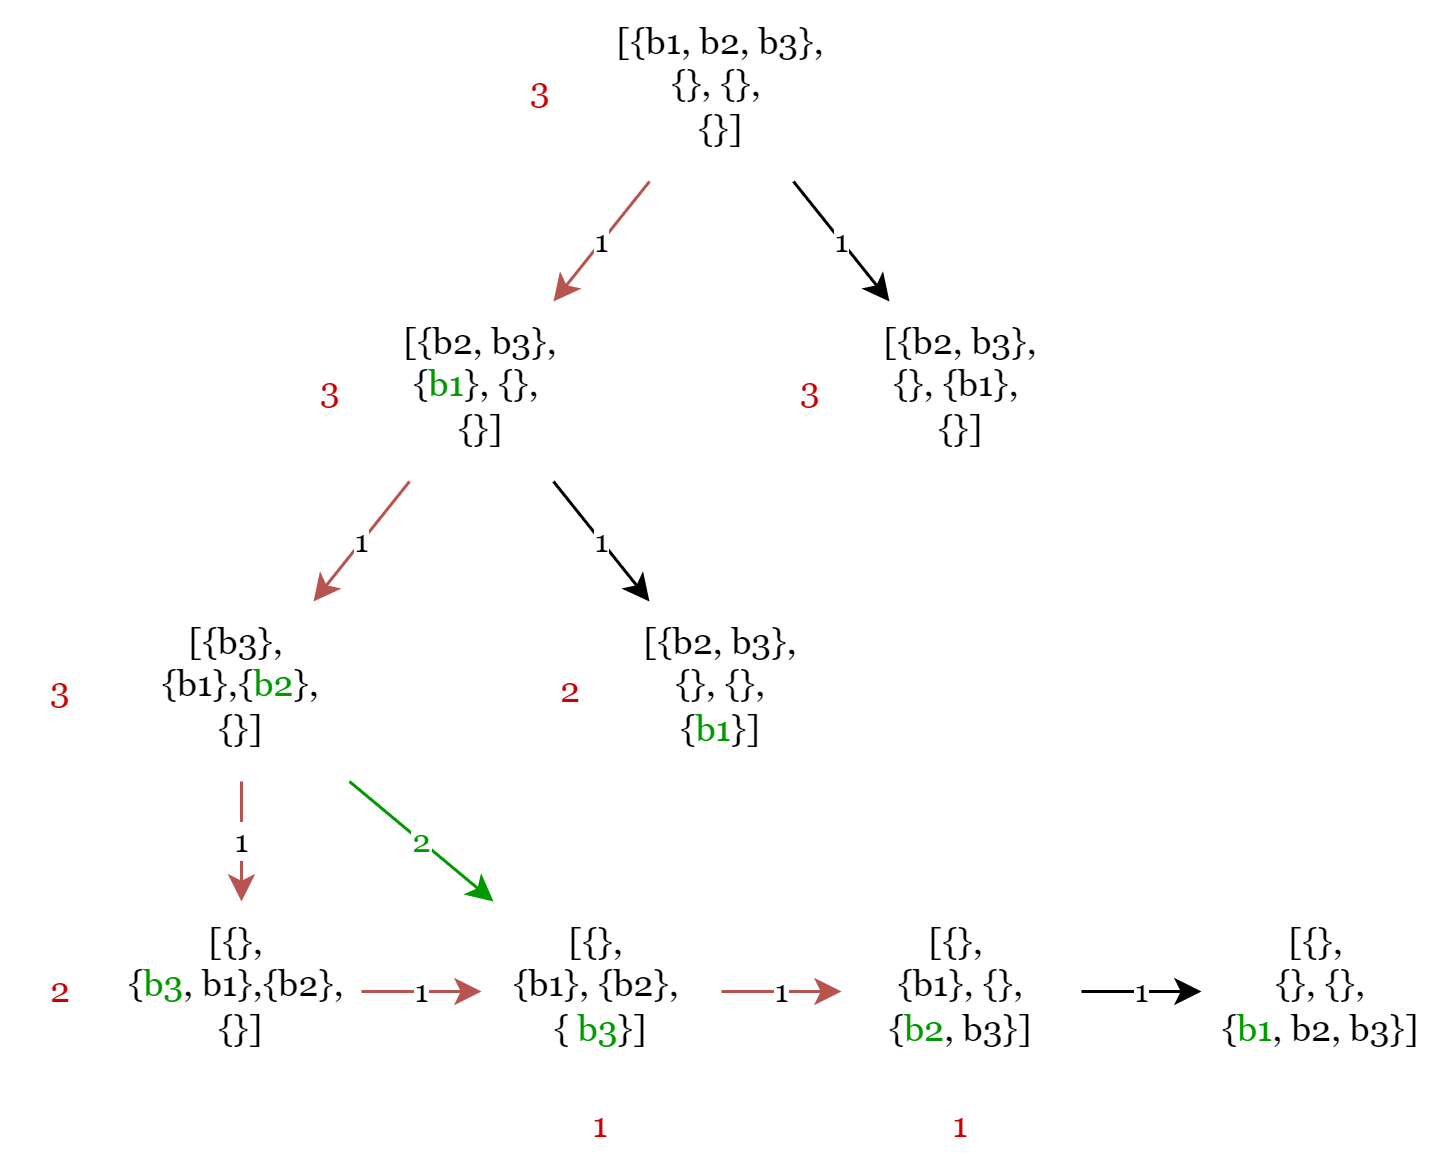
\includegraphics[scale=0.25]{"./Diagrams/DFS_Tree_Solution.png"}
        \end{center}
        The solution is shown by the red arrows. The cost of each action is shown in the arrow as black text, and the red text represents the heuristic of each state. The green elements highlights the box that is currently held by the mover. There is a green arrow which represents a "shortcut" as the mover moves from $a$ to $d$ through $c$. Note that in $[\{\}, \{b_3, b_1\}, \{b_2\}, \{\}]$ the order rule appears to be violated as $b_3$ is above $b_1$. But since the box $b_3$ is being held by the mover in room $b$, it is not violated.
  \item How would the state representation change in part A if the following modifications are applied to the problem:
        \begin{itemize}
          \item The cost to move one box is now proportional to the size of the box (cost of 1 for moving the smallest box, cost of 3 for moving the largest one).
          \item If the moving company employee moves from one corner to the other without carrying any box, it also incurs a cost of 0.5
        \end{itemize}
        For my state representation, the box representation will still work as my boxes are labelled as $b_i$ where $i$ is the weight. Similarly, the position of the mover is still the same with the new rule that movement from one corner to another without a box will cost 0.5.\\[10pt]
        The changes can be seen in the \textbf{actions} rather than in the state. Now we can redefine an action to $C(a,b,b_i)$, where the mover moves a box $b_i$ from room $a$ to $b$. Previously the cost was $1$ for any $b_i$ but the new cost will be $i$.\\
        Another change we have to make is to represent the position of the mover. Previously I ignored his position in our state representation as his movement cost without a box was 0. But now, we can have a new action $C(a,b,b_0)$ which costs 0.5, when a mover moves from room $a$ to room $b$ without a box. Now we cannot ignore the position of the mover, and we require an additional variable in our state $m$ to represent the room the mover is currently in.
\end{enumerate}